\section{Apresentação}

\begin{frame} % Capa
    \titlepage
\end{frame}

\begin{frame}{Apresentação}
    \begin{itemize}
        \item Professor {\fontfamily{augie}\selectfont Rodrigo de Farias Gomes}
        \item Telefone (somente mensagens): (92) 9 9405-1724
        \item E-mail: shpnft@gmail.com

    \end{itemize}

    \centering

    \vspace{2cm}
    \begin{tabular}{cccccc}
        R & G & O & M & E & S \\ \\
        \(\color{red} \left.\phantom{{\scriptstyle +1}\frac{1}{2}}\right\downarrow {\scriptstyle +1}~~\) &
        \(\color{red} \left.\phantom{{\scriptstyle +1}\frac{1}{2}}\right\downarrow {\scriptstyle +1}~~\) &
        \(\color{red} \left.\phantom{{\scriptstyle +1}\frac{1}{2}}\right\downarrow {\scriptstyle +1}~~\) &
        \(\color{red} \left.\phantom{{\scriptstyle +1}\frac{1}{2}}\right\downarrow {\scriptstyle +1}~~\) &
        \(\color{red} \left.\phantom{{\scriptstyle +1}\frac{1}{2}}\right\downarrow {\scriptstyle +1}~~\) &
        \(\color{red} \left.\phantom{{\scriptstyle +1}\frac{1}{2}}\right\downarrow {\scriptstyle +1}~~\) \\ \\
        S & H & P & N & F & T
    \end{tabular}
\end{frame}

\begin{frame}{Calendário}
    \centering
    \small{
        \begin{tabular}{cP{2cm}P{2cm}P{2cm}P{2cm}P{2cm}}
            \rowcolor{black!10} & Segunda & Terça & Quarta & Quinta & Sexta \\
            01 & \dma{0} & \dma{1} & \dma{2} & \dma{3} & \dma{4} \\
            02 & \dma{7} & \dma{8} & \dma{9} & \dma{10} & \dma{11} \\
            03 & \dma{14} & \dma{15} & \dma{16} & \dma{17} & \dma{18} \\
            04 & \dma{21} & \dma{22} & \dma{23} & \dma{24} & \dma{25} \\
            05 & \dma{28} & \dma{29} & \dma{30} & \dma{31} & \dma{32} \\
            06 & \dma{35} & \dma{36} & \dma{37} & \dma{38} & \dma{39} \\
            07 & \dma{42} & \dma{43} & \dma{44} & \dma{45} & \dma{46} \\
            08 & \dma{49} & \dma{50} & \dma{51} & \dma{52} & \dma{53} \\
            09 & \dma{56} & \dma{57} & \dma{58} & \dma{59} & \dma{60} \\
            10 & \dma{63} & \dma{64} & \dma{65} & \dma{66} & \dma{67} \\
            11 & \dma{70} & \dma{71} & \dma{72} & \dma{73} & \dma{74} \\
            12 & \dma{77} & \dma{78} & \dma{79} & \dma{80} & \dma{81} \\
            13 & \dma{84} & \dma{85} & \dma{86} & \dma{87} & \dma{88} \\
            14 & \dma{91} & \dma{92} & \dma{93} & \dma{94} & \dma{95} \\
            15 & \dma{98} & \dma{99} & \dma{100} & \dma{101} & \dma{102} \\
            % 16 & \dma{103} & \dma{104} & \dma{105} & \dma{106} & \dma{107} \\
            % 17 & \dma{108} & \dma{109} & \dma{110} & \dma{111} & \dma{112} \\
        \end{tabular}
    }
\end{frame}

\begin{frame}{Meus horários em 20/03/2023...}
    \small{
        \begin{center}
            \begin{tabular}{ccccc}
                \rowcolor{black!10} Segunda & Terça & Quarta & Quinta & Sexta \\ \hline
                \rowcolor{red!25} &&&& \\ \hline
                \rowcolor{red!25} Métodos Num... & Trigonometria & Métodos Num... & Trigonometria & \\ \hline
                \rowcolor{green!25} & & Termodinâmica & & Termodinâmica \\ \hline
                \rowcolor{green!25} & Óptica e Eletro... & & Óptica e Eletro... & \\ \hline
                \rowcolor{blue!25} &&&& \\ \hline
                \rowcolor{blue!25} &&&& \\ \hline
            \end{tabular}
        \end{center}

        \vspace{1cm}
        Legenda:
        \begin{itemize}
            \item[\textcolor{red!25}{\rule{1em}{1em}}] Manhã (8:00 -- 10:00 e 10:00 -- 12:00)
            \item[\textcolor{green!25}{\rule{1em}{1em}}] Tarde (14:00 -- 16:00 e 16:00 -- 18:00)
            \item[\textcolor{blue!25}{\rule{1em}{1em}}] Noite (18:00 -- 20:00 e 20:00 -- 22:00)
        \end{itemize}
    }
\end{frame}


\begin{frame}{Ementa de \Disciplina}
    \begin{itemize}
        \item Trigonometria no Triângulo Retângulo
            \begin{itemize}
                \item Teorema de Pitágoras
                \item Razões trigonométricas no triângulo retângulo
            \end{itemize}
        \item Trigonometria na Circunferência
            \begin{itemize}
                \item Arcos e ângulos
                \item Razões trigonométricas na circunferência
                \item Relações fundamentais
            \end{itemize}
        \item Funções Trigonométricas
            \begin{itemize}
                \item Funções seno, cosseno, tangente \textit{et al}
                \item Transformações e identidades
                \item Equações e inequações
                \item Funções inversas
            \end{itemize}
    \end{itemize}
\end{frame}

\begin{frame}{Avaliação}
    \begin{itemize}
        \item A avaliação será na forma de 3 notas: \(N_1\), \(N_2\) e \(N_3\)
        \item A média dos exercícios escolares (\(MEE\)) será dada por
            \[
                MEE=\frac{N_1+N_2+N_3}{3}
            \]
        \item Se \(MEE \geq 8,0\), então a média final (\(MF\)) será igual à \(MEE\)
        \item Se \(MEE < 8,0\), então
            \[
                MF=\frac{2\times MEE+PF}{3}
            \]
            onde PF é a nota da \textbf{prova final}
        \item Se \(MF \geq 5,0\) e a frequência em sala for maior que 75\%, o aluno está aprovado
        \item Haverá 30 aulas de \SI{2}{horas}, de forma que \textbf{o número máximo de faltas é 8}
    \end{itemize}
\end{frame}

\begin{frame}{Livro}
    \centering
    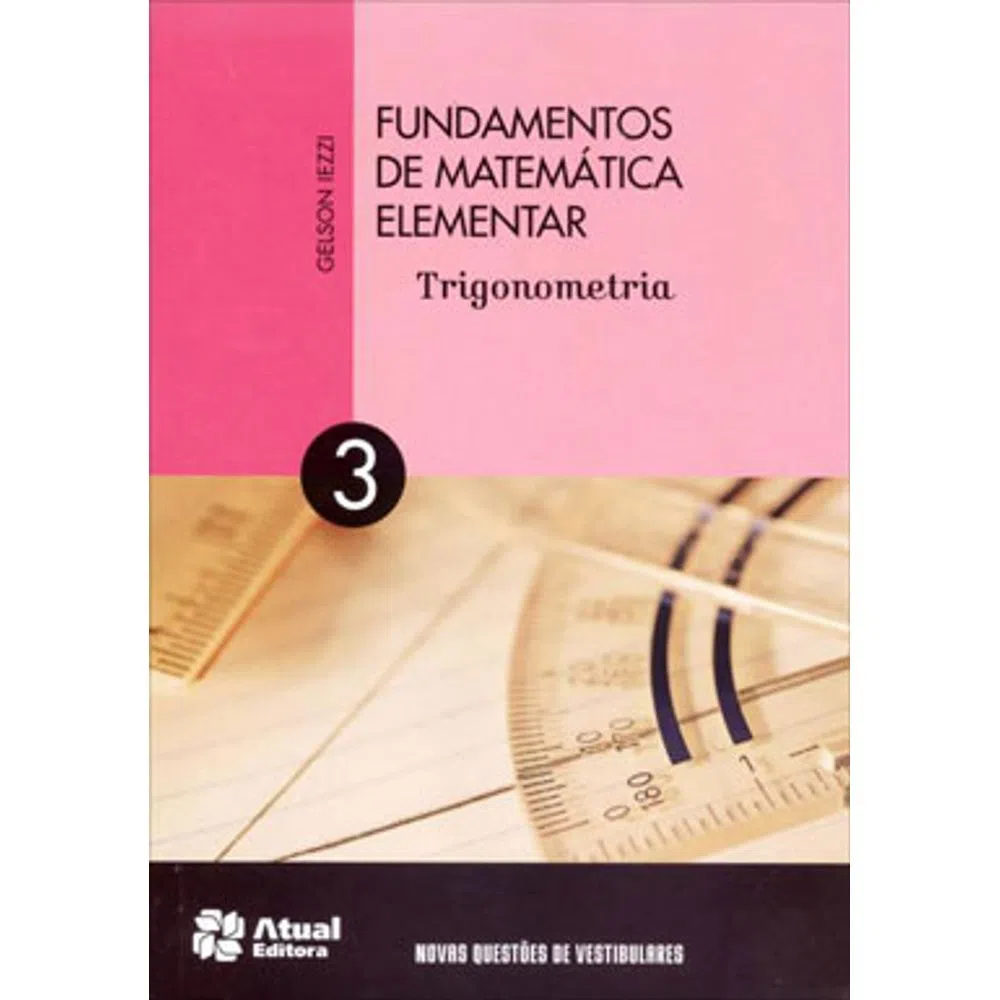
\includegraphics[height=0.8\textheight]{images/iezzi.png}
\end{frame}
